\fontfamily{\sfdefault}\selectfont
% XCircuit output "div_noise_model.tex" for LaTeX input from div_noise_model.ps
\def\putbox#1#2#3#4{\makebox[0.00000in][l]{\makebox[#1][l]{}\raisebox{\baselineskip}[0.00000in][0.00000in]{\raisebox{#2}[0.00000in][0.00000in]{\scalebox{#3}{#4}}}}}
\def\rightbox#1{\makebox[0.00000in][r]{#1}}
\def\centbox#1{\makebox[0.00000in]{#1}}
\def\topbox#1{\raisebox{-0.60\baselineskip}[0.00000in][0.00000in]{#1}}
\def\midbox#1{\raisebox{-0.20\baselineskip}[0.00000in][0.00000in]{#1}}
   \scalebox{1}{
   \normalsize
   \parbox{2.75260in}{
   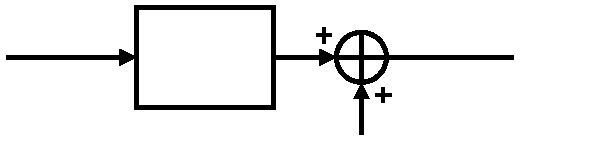
\includegraphics[scale=0.70000]{./figs/div_noise_model.pdf}\\
   % translate x=-96 y=524 scale 0.38
   \putbox{0.04200in}{0.53200in}{1.20}{$\Phi_{out}$[n]}%
   \putbox{0.79800in}{0.39200in}{1.20}{$\div \mathrm{N}$}%
   \putbox{1.74300in}{0.05600in}{1.20}{$\Phi_{n_{div}}$}%
   \putbox{1.84800in}{0.53200in}{1.20}{$\Phi_{div}$[n]}%
   } % close 'parbox'
   } % close 'scalebox'
   \vspace{-\baselineskip} % this is not necessary, but looks better
\fontfamily{\rmdefault}\selectfont
